\documentclass{article}

% if you need to pass options to natbib, use, e.g.:
%     \PassOptionsToPackage{numbers, compress}{natbib}
% before loading neurips_2018

% ready for submission
% \usepackage{neurips_2018}

% to compile a preprint version, e.g., for submission to arXiv, add add the
% [preprint] option:
%     \usepackage[preprint]{neurips_2018}

% to compile a camera-ready version, add the [final] option, e.g.:
     \usepackage[final]{nips_2018}

% to avoid loading the natbib package, add option nonatbib:
%     \usepackage[nonatbib]{neurips_2018}

\usepackage[utf8]{inputenc} % allow utf-8 input
\usepackage[T1]{fontenc}    % use 8-bit T1 fonts
\usepackage{hyperref}       % hyperlinks
\usepackage{url}            % simple URL typesetting
\usepackage{booktabs}       % professional-quality tables
\usepackage{amsfonts}       % blackboard math symbols
\usepackage{nicefrac}       % compact symbols for 1/2, etc.
\usepackage{microtype}      % microtypography
\usepackage{graphicx}
\usepackage{titlesec}

\hypersetup{
    colorlinks=true,
    linkcolor=blue,
    filecolor=magenta,      
    urlcolor=cyan,
}

\title{Automatic Image Captioning through Neural Networks and Exploring the Possibility of Image Captioning Model on Mobile Devices}

% The \author macro works with any number of authors. There are two commands
% used to separate the names and addresses of multiple authors: \And and \AND.
%
% Using \And between authors leaves it to LaTeX to determine where to break the
% lines. Using \AND forces a line break at that point. So, if LaTeX puts 3 of 4
% authors names on the first line, and the last on the second line, try using
% \AND instead of \And before the third author name.

\author{%
  Jilin Cao \\
  University of California, Berkeley\\
  \texttt{caojilin@berkeley.edu} \\
  \And
  Mike Jin \\
  University of California, Berkeley\\
  \texttt{mikejin@berkeley.edu} \\
  \And
  Daniel Kim \\
  University of California, Berkeley\\
  \texttt{danieljkim@berkeley.edu} \\
  \And
  Zabin Bashar \\
  University of California, Berkeley\\
  \texttt{zabin326@berkeley.edu} \\
  % examples of more authors
  % \And
  % Coauthor \\
  % Affiliation \\
  % Address \\
  % \texttt{email} \\
  % \AND
  % Coauthor \\
  % Affiliation \\
  % Address \\
  % \texttt{email} \\
  % \And
  % Coauthor \\
  % Affiliation \\
  % Address \\
  % \texttt{email} \\
  % \And
  % Coauthor \\
  % Affiliation \\
  % Address \\
  % \texttt{email} \\
}

\begin{document}
% \nipsfinalcopy is no longer used

\maketitle

\begin{abstract}
The recent development of machine translation and object detection via Neural Networks motivated us to construct a model that automatically learns the contents of images and interprets them in human languages. In particular, we trained an attention-based model that extracts features from images through Convolutional Neural Networks and decodes the information into natural sentences through Recurrent Neural Networks. Our model achieved state-of-the-art results on Flickr8K and MSCOCO datasets. In addition, we experimented with different pre-trained Convolutional Neural Network models as our encoders and evaluated their performances on these two datasets. Finally, we explored some future applications of image-captioning model and the possibility of putting the model into mobile phone applications.
\end{abstract}

\section{Introduction}

As photo-taking becomes more convenient and prevalent nowadays, it is not surprising that an ordinary person would have thousands of images storing on his or her computer and phone. However, most of the images are disorganized, and while there are platforms such as \textit{Google Photos} and Apple’s \textit{Photos} that automatically create categories for images, such labels only consist of single words, as opposed to complete sentences. Hence, searching for an image with complicated phrases or broken sentences is not allowed on these platforms, which makes the task of pinpointing a specific image in mind much more difficult and time-consuming.

In this project, we would like to utilize the power of Neural Networks to propose an image-captioning model that could identify objects in an image and produce a caption that accurately describes the image. In the past, automatic caption generation has long been regarded as a challenging task because we needed a very powerful model that not only captures different articles in an image but also express the relationships among these objects in natural and logical languages. As the technology of Neural Networks becomes more advanced, we were able to combine Convolutional Neural Network models such as ResNet, VGG, SqeeuezeNet, and MobileNet, with Recurrent Neural Network architectures such as LSTM to propose a solution to the image-captioning task through this powerful and effective encoder-decoder framework.

In addition, we incorporated the well-known attention mechanism, which serves as an active direction of the mind to an object and helps Neural Networks make choices about where and what they pay attention to. Our experiments indicated a significant improvement in our model when the attention mechanism was added.

Finally, beyond coming up with a model that can tackle the traditional image captioning problem, we would also like to put our focus on investigating the potential feasibility of inserting our model into mobile phone applications. This is definitely more challenging because this would require not only high prediction accuracy but also small model size so that it can be run on small devices. In other words, we needed to find the perfect balance between the accuracy and the speed of the model. 

\section{Related Work}
\label{rel_work}

In this section, we provide relevant information on the background of the image caption generation. One of the early methods of tackling image caption was to learn separate representations for each of the modalities and then sew them with regards to some constraints. Well-suited choice of constraint is similarity, either in the sense of cosine distance (Weston et al., 2011; Frome et al., 2013) or the Euclidean distance.

A more advanced method developed by adopting Recurrent Neural Network models. The image caption generation is effectively laid out by the encoder-decoder framework (Cho et al., 2014). The challenge of generating caption is similar to translating an image to a sentence. Past studies have adopted the Recurrent Neural Networks model with sequence-to-sequence machine translating for this method. A multimodal log-bilinear model was proposed by Kiros et al. (2014a). Mao et al. (2014) replaced the feed-forward neural language model with a recurrent model. Both Vinyals et al. (2014) and Donahue et al. (2014) use LSTM RNNs for their models.

Instead of regarding images as a single feature vector from the top layer of a pre-trained convolutional network, Karpathy \& Li (2014) proposed a combination of CNNs over image regions, bidirectional RNNs over sentences, a multimodal embedding that aligns the two modalities. Vinyals et al. (2014) similarly proposed a concept of Neural Image Caption which is a concept of using CNN as an image encoder, by first pre-training it for an image classification task and using the last hidden layer as an input to the RNN decoder. 

% The test results from these two papers will serve as the references to the accuracy of our model. 

\section{Dataset and Features}
\label{dataset}

We trained our models using the Microsoft COCO dataset, which contains 123,287 images. Each image has five human-annotated captions that describe the image. We use 83,000 images for training and 41,000 images for validation. An example from the dataset is shown above in Figure 1. The reason why we found the dataset with 5 captions per image useful was that we would like to catch the subtleties of the image, as each caption has a somewhat different focus on the image.

\begin{figure}
\graphicspath{ {./images/} }
    \centering
    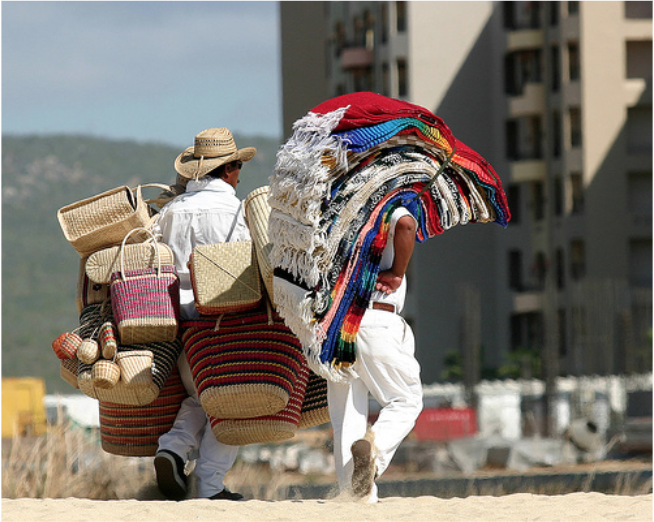
\includegraphics[scale=0.32]{Image}
    \hspace{0.5cm}
    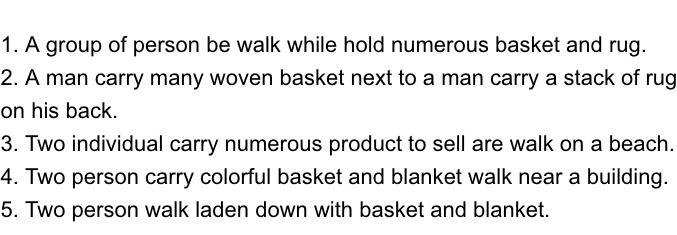
\includegraphics[scale=0.4]{dataset2}
    \caption{Sample image and captions}
    \label{fig:my_label}
\end{figure}

In order to help our model to learn the captions efficiently, we went through the preprocessing stage by using several tokens. Each caption starts with a <start> token and ends with a <end> token. These two tokens, while obvious, are indeed very important because we need to tell our model to generate the first word and also make them learn to predict the end of a caption, in other words, our model needs to learn when to stop decoding during the inference stage. 

Because we would like to input the captions at the fixed size into our model, we used the  <pad> token to make sure that every caption is of the same length. Finally, for words with a frequency of less than our preset threshold (for example, less than five times, but our threshold is really depended on the size of our dataset) are replaced with <unk> token, which stands for “unknown”. Every word and token is mapped into numbers which we can treat them as inputs and outputs of our learning model. For instance, <start> a man holds a football <end> <pad> <pad> <pad>... are mapped into numbers 9876 1 5 120 1 5406 9877 9878 9878 9878...

\section{Model}

\subsection{Model Architecture}
\graphicspath{ {./images/} }
\begin{figure}[!htb]
    \centering
    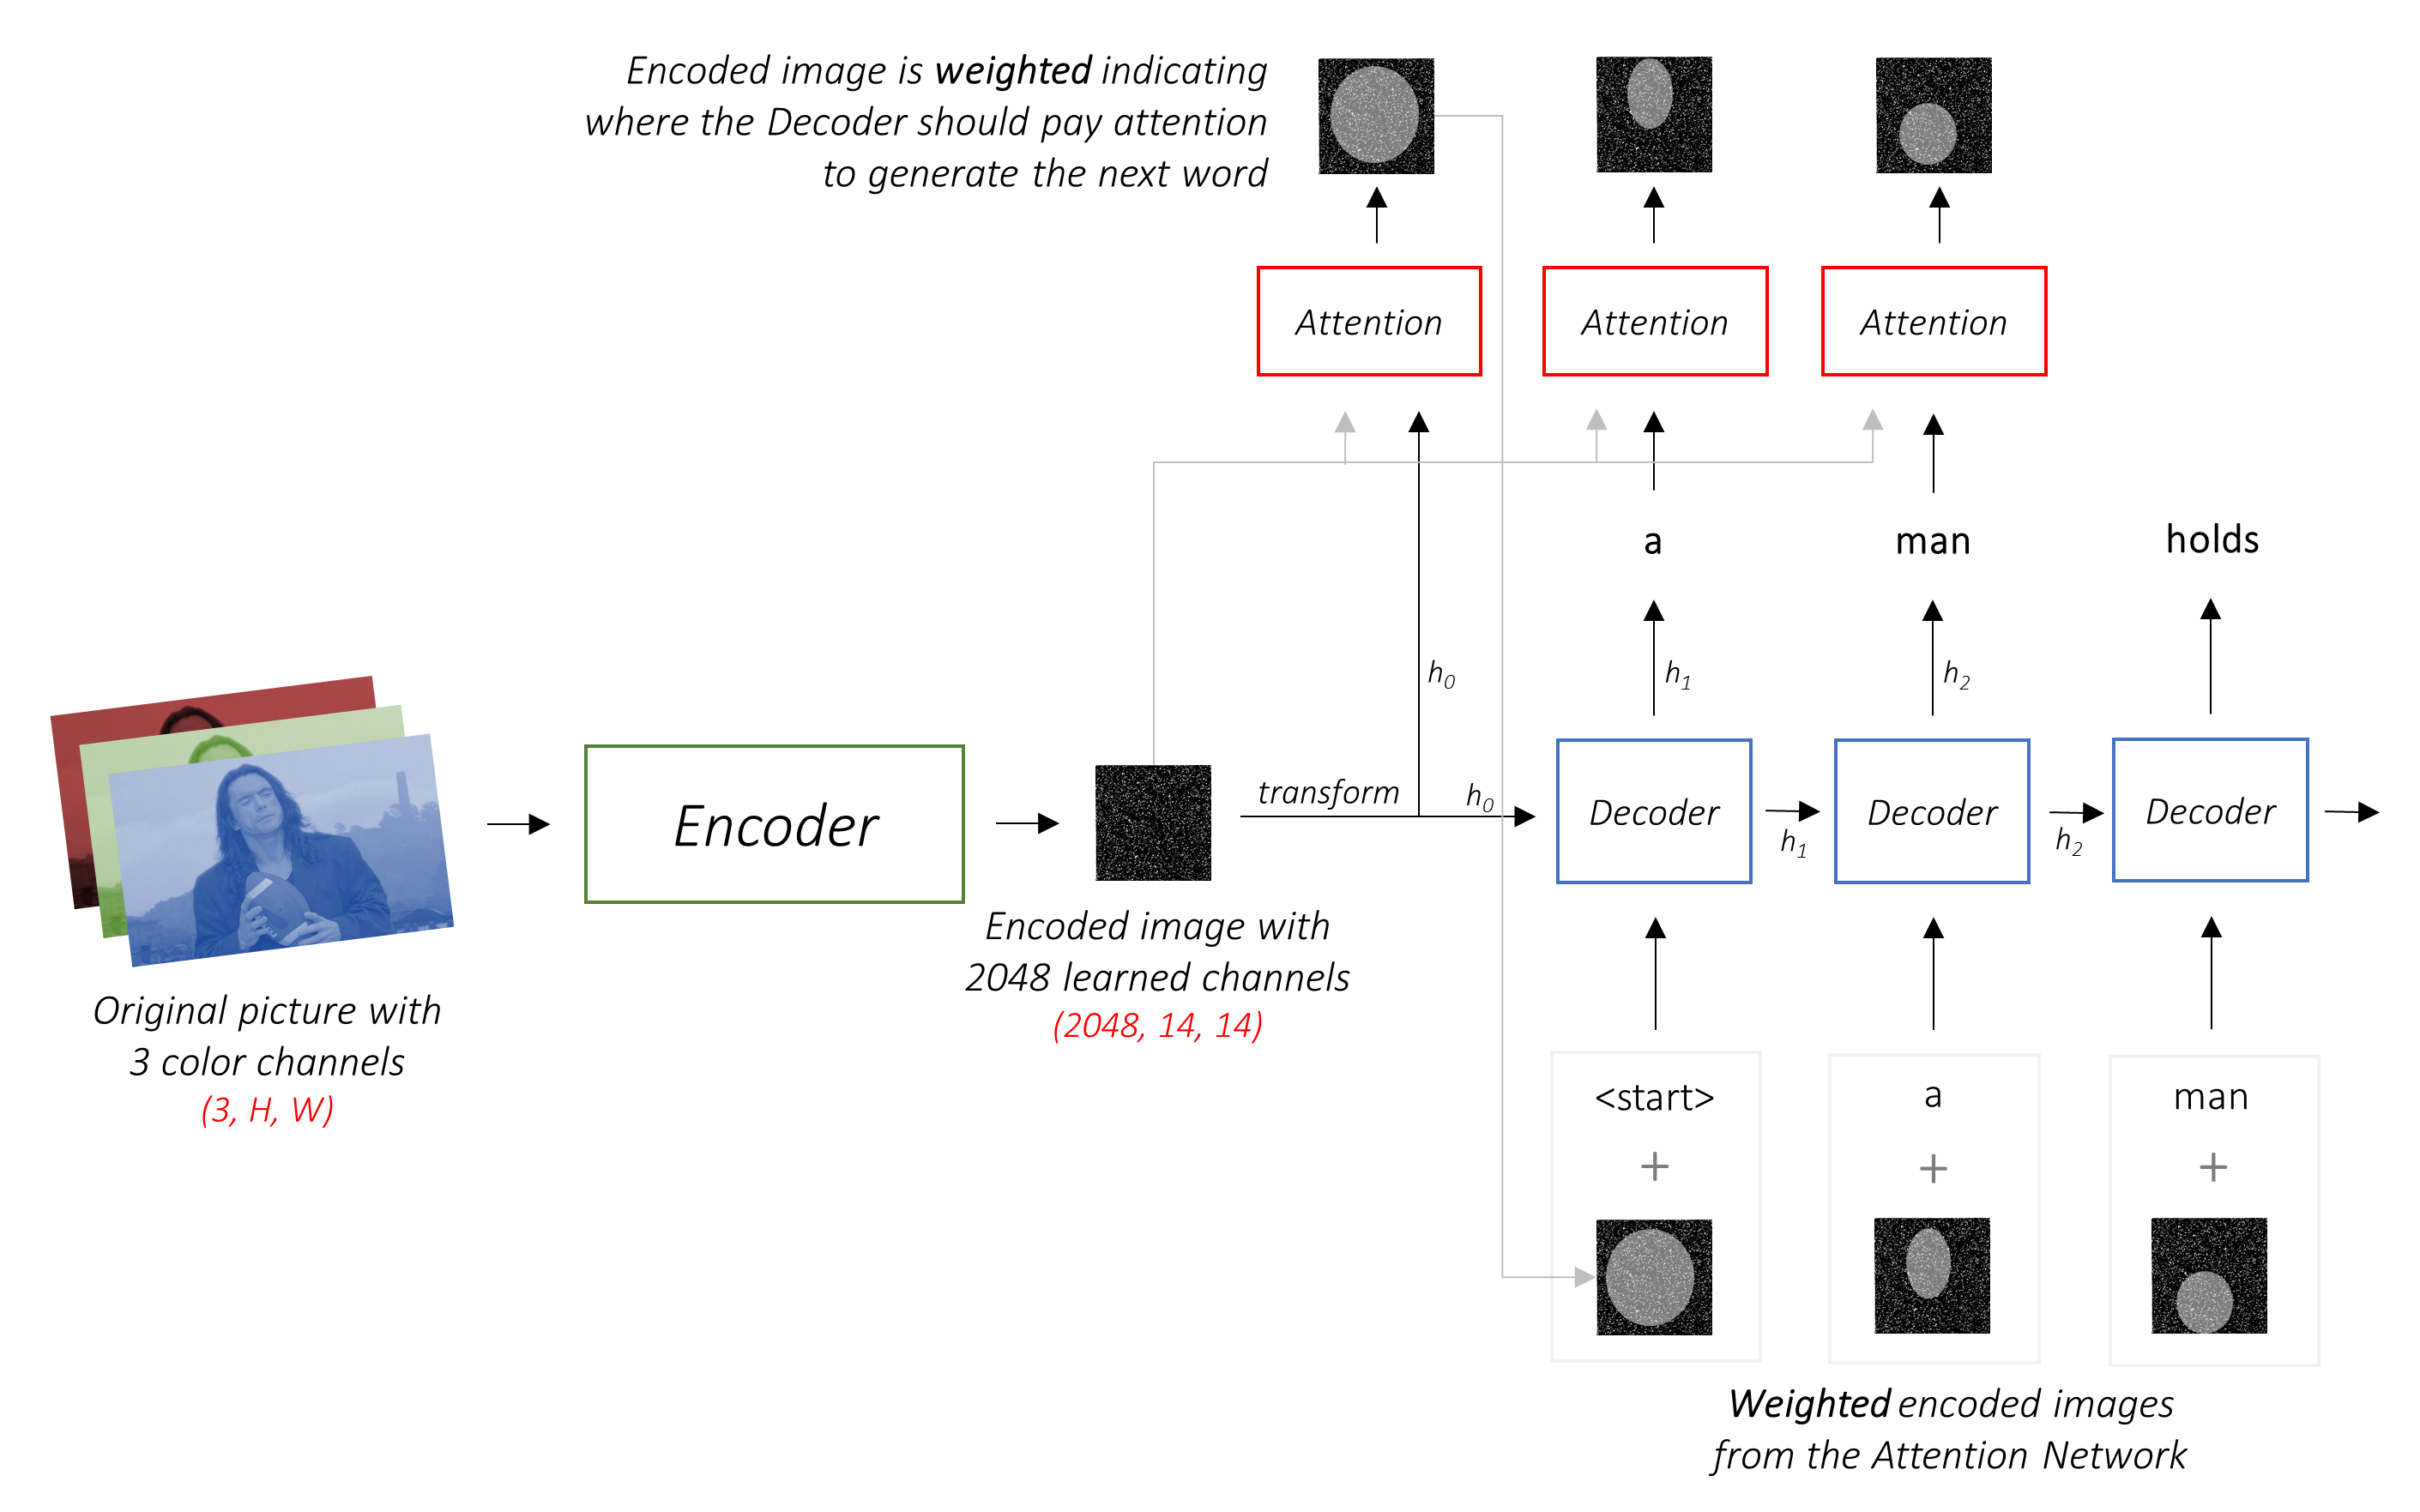
\includegraphics[scale=0.5]{images/model.png}
    \caption{Stages of encoding and decoding}
    \label{fig:my_label}
\end{figure}

First, we drop the last layer of a pre-trained ImageNet model such as Residual Network, VGG, and use only the output from last convolutional block to create image embedding vectors. Then we feed these features along with each word to an attention network to weight these features of the image. We use weighted features instead of raw features generated from encoder, because the attention network can help focus processing on only the most informative parts of the input hence improving accuracy. An example of this process is displayed in Figure 3 where white colored region represents the weighted area.

\graphicspath{ {./images/} }
\begin{figure}[!htb]
    \centering
    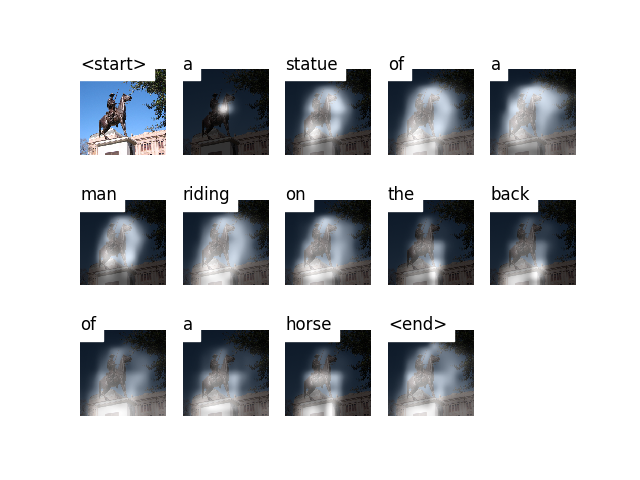
\includegraphics[scale=0.5]{images/lstmex.png}
    \caption{LSTM example with attention mechanism}
    \label{fig:my_label}
\end{figure}

We use image feature vectors transformed by a gated recurrent activation function as the initial hidden state of the LSTM. We used the word embedding network to create the word embeddings that are used by the LSTM when generating the caption. We chose an LSTM because it has expressive multiplicative interactions, gradients flow nicely, and the network can now explicitly decide to reset the hidden state. At each time-step of generating the caption, the LSTM considers the previous cell state and outputs a prediction for the most probable next word value until an end token is sampled to signal the end of the caption.

\subsection{Loss Function}

Since we would like to compare the generated sequences with the target sequences, we used the Cross-Entropy loss as shown here:

\begin{equation} Loss(y, \hat{y}) = -\sum_{i=0}^n y_{i}\log{\hat{y_{i}}}
\end{equation}

In addition, in order to regularize our attention network, we used a second loss function called the“doubly stochastic regularization”, which is introduced in Kelvin Xu et al. (2016)’s paper. While we knew that the weights are summed to 1 at a given timestep, we also wanted to encourage the weights at a single pixel p to sum to 1 across all timestep T. That is:

\begin{equation} 
\sum_{t=0}^T \alpha_{p, t} = 1
\end{equation}

This means that we needed our model to pay attention to every pixel over the course of generating the entire sequence. Therefore, we tried to minimize the difference between 1 and the sum of a pixel’s weights across all timesteps.

\subsection{Training}

Training our model from scratch can be extremely expensive in terms of time and money. So, we exploited some of the pre-trained models on ImageNet. We believed that these pre-trained models are powerful enough to extract necessary features from a given image. 

With the help of these pre-trained models, we can just do fine-tuning on the encoder. Thus, we need a very small learning rate for encoder training. Due to the complexity of the model and the size of datasets, we started the training without the fine-tuning at the beginning, and after the model’s update was slowing down, we switched back to the fine-tuning. We found out that after turning on the fine-tuning, the model’s performance increased significantly.

Nevertheless, we still have to train the decoder from scratch because we did not possess prior knowledge about our datasets. As we have seen from the analysis of different models, the decoder with attention usually has more parameters than the encoder, in which we used Adam optimizer with an initial learning rate of 4e-4.

\subsection{Early Stopping}

Kelvin Xu et al. (2016) observed that the correlation between the loss and the BLEU score breaks down after a certain point; thus, it is recommended that we stop our training early on when the BLEU score begins to degrade, even if the loss continues to decrease. Although there exists a considerable amount of criticism on the BLEU metrics because it doesn’t always correlate well with human consensus, it is still an informative metric for machine translate evaluation. As a result, after every epoch, we evaluated BLEU-4 score on the validation datasets, and after we observed a decrease in the score, we stopped training.


\section{Experiment}

\subsection{Evaluation Metrics}

Unlike ordinary regression and classification, for image captioning, there is no such metric that takes in a prediction as input and spits out a number to represent the absolute accuracy that is universally recognized. Evaluation metrics regarding image captioning are more subjective: how a model performs in producing a sequence of words not only depends on the model itself but also relates to what kind of metrics it has been testing on. Therefore, it is fairly important to choose the right metrics that can properly measure the performance of our image-captioning model.

After researching on many metrics in the field of NLP tasks, we decided on using the following ones to evaluate the results of our model:

\begin{itemize}
    \item \textbf{BLEU-n} is one of the earliest and the most popular metrics for evaluating sequence to sequence tasks. Basically, it looks at the n-grams overlap between our model’s outputs and reference translations, in our case, the captions in our validation set. However, BLEU has some major drawbacks, for example, it does not consider sentence structures, nor word meanings.
    \item \textbf{Meteor} is a metric that is very similar to BLEU but includes additional features. It not only considers the synonyms but also compares the outputs to the stems of words, so that “running”, “runs”, and “run” would be regarded as the same word, hence counting as matches. As a result, these extra focus of Meteor makes it a better choice in evaluating sentences.
    \item \textbf{Rouge} is a modification of BLEU that focuses on recall rather than precision. In other words, it looks at how many n-grams in the reference translations show up in our outputs, rather than the other way around. However, in this case, Rouge is more biased towards long sentences in our predictions because they will have higher chance in containing the targeted words and phrases.
    \item \textbf{CIDEr}, also known as the \textit{Consensus-based Image Description Evaluation}, is the latest and a more complicated metric that measures the similarity of a generated sentence against a set of ground truth sentences written by humans. 
\end{itemize}

\subsection{Model Performance}
\begin{table}[!htbp]
\centering
  \caption{Model Performance on COCO dataset: B-n stands for BLEU-n, M stands for METEOR, R-L stands for ROUGE-L, C stands for CIDEr.}
  \label{model-table}
  \centering
  \begin{tabular}{llllllll}
    \toprule
    Encoder Model & B-1 & B-2 & B-3 & B-4 & M & R-L & C \\
    \midrule
    ResNet-101 & \textbf{73.2} & \textbf{56.6} & \textbf{43.3} & \textbf{33.2} & \textbf{26.0} & \textbf{54.5} & \textbf{104.2}\\
    VGG-16 & 72.5 & 56.0 & 42.6 & 32.4 & 25.2 & 53.5 & 98.4\\
    MobileNet & 71.6 & 55.0 & 41.6 & 31.4 & 24.9 & 53.1 & 97.0\\
    SqueezeNet & 60.9 & 42.8 & 30.4 & 22.2 & 19.2 & 45.4 & 60.1\\
    \midrule
    Karpathy et al. (2015) & 62.5 & 45.0 & 32.1 & 23.0 & 19.5 & N/A & 66.0\\
    Xu et al. (2016) & 71.8 & 50.4 & 35.7 & 25.0 & 23.0 & N/A & N/A\\
    \bottomrule
  \end{tabular}
\end{table}

\begin{table}[!htbp]
\centering
  \caption{Model Efficiency on COCO dataset: Param-EN stands for number of parameters in the encoder, Param-DE stands for number of parameters in the decoder, BM-n stands for beam search size = n.}
  \label{model-table}
  \centering
  \begin{tabular}{lllllllll}
    \cline{5-9}
    & & & & \multicolumn{5}{|c|}{Number of Predictions Per Second}\\
    \toprule
    Encoder Model & Size & Param-EN & Param-DE & BM-1 & BM-2 & BM-3 & BM-4 & BM-5\\
    \midrule
    ResNet-101 & 720M & 42,500,160 & 20,483,859 & 19.73 & 16.02 & 14.81 & 13.85 & 12.39\\
    VGG-16 & 332M & 14,723,136 & 14,190,867 & 24.37 & 20.02 & 18.95 & 18.50 & 16.74\\
    MobileNet & 224M & 3,206,976 & 16,288,531 & 38.20 & \textbf{29.79} & \textbf{27.26} & 23.58 & 21.85\\
    SqueezeNet & \textbf{200M} & \textbf{1,235,496} & \textbf{16,190,203} & \textbf{39.58} & 28.70 & 26.29 & \textbf{24.67} & \textbf{22.56}\\
    \bottomrule
  \end{tabular}
\end{table}

The performances of our four encoding models can be seen in Table 1. Each model strictly dominates in terms of performance over the models listed below them. ResNet-101 was the best performing model and SqueezeNet was the worst performing model out of the four that we experimented on. From Table 1, we can also see that our best performing model, which used ResNet-101 as its encoder, not only shows a significant improvement from the original image captioning model proposed by Karapathy et al. in 2015 but also beats the state-of-the-art hard attention model proposed by Kevin Xu et al. in 2016 in every evaluation category. While our model is not yet "the best" in the field of image captioning, we believe that we can improve the model if we can obtain better training resources in the future.

In terms of efficiency, VGG-16 has a overwhelming advantage over ResNet-101, as ResNet-101’s model size is twice as large as the size of VGG-16, yet their performances are very close to each other. This explains why people usually use VGG model on neural style transfer instead of using ResNet, which has better performance on image classification. As we know that VGG is better in extracting features than ResNet, hence, for large-scale data processing, we prefer to use the VGG model. In our experiment, we only trained VGG-16 because we want to make sure our training process would not take too long. However, in future works, we would like to incorporate the VGG model with more layers. 

While MobileNet and SqueezeNet are both designed to have a smaller model size, we found our that MobileNet is more powerful in extracting features than SqueezeNet, despite having 3 million parameters while SqueezeNet only has 1.2 million parameters. For the purpose of finding a suitable model for mobile applications, we find that MobileNet and VGG will fit our needs.

Traditionally, people use a greedy algorithm to find the best sequence – at each timestep, we pick the word with the highest score. However, simply choosing the words with the best score at each decode-step does not necessarily yield the optimal sequence. Beam Search allows us to find the most optimal sequence by maintaining a top k list of sequences, and then we can pick the best sequence in the end. Note that Beam size 5 is usually enough for generating optimal sequences.

\graphicspath{ {./images/} }
\begin{figure}[!htbp]
    \centering
    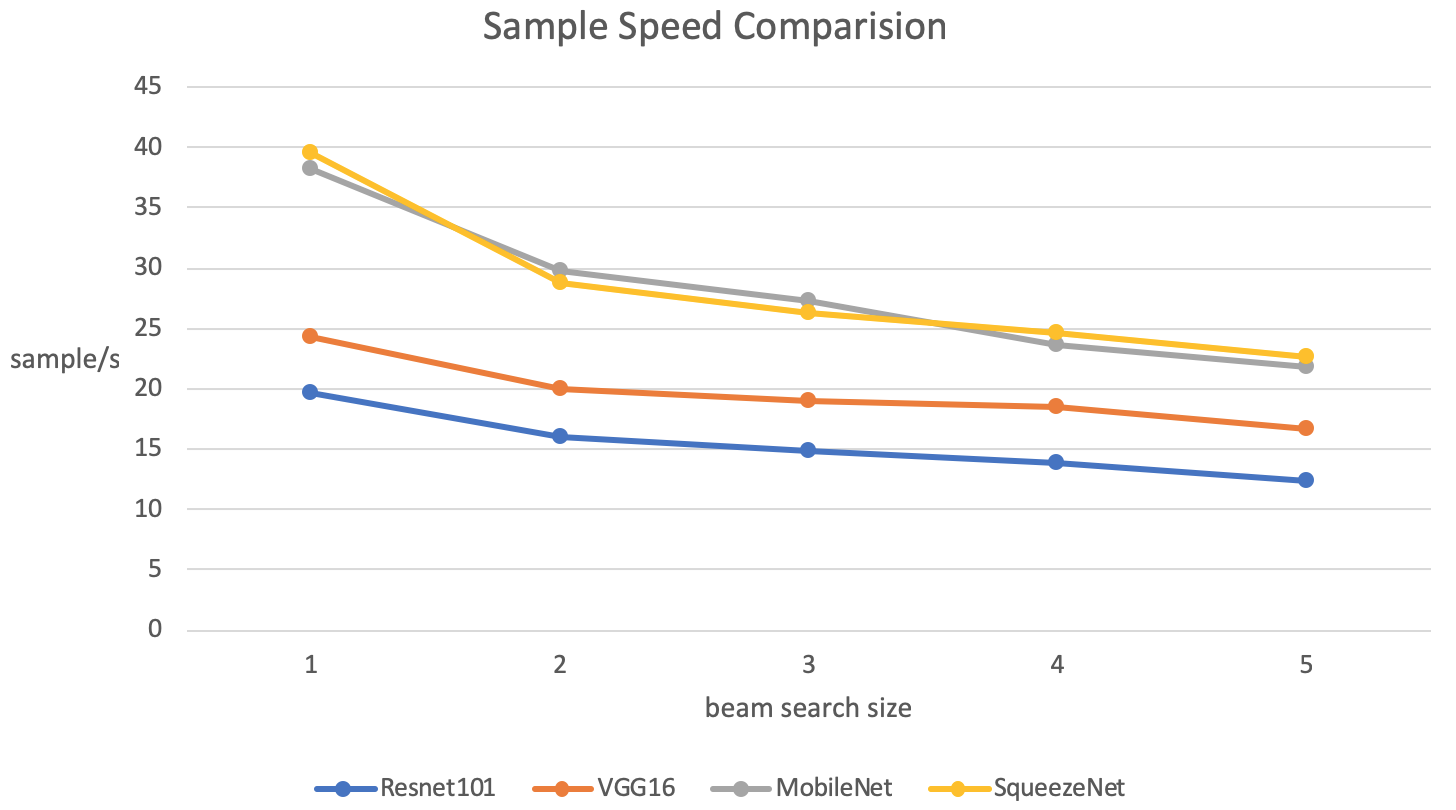
\includegraphics[scale=0.4]{graph}
    \caption{Sample speed comparison between models with different beam search size}
    \label{fig:my_label}
\end{figure}

However, there is a trade-off between beam size and sampling speed. Thus, we compared different beam size on different models. As we can see in Table 2 and the above figure, there is a negative relationship between beam size and sampling speed; in other words, increasing beam size will reduce sampling speed. While there is no clear speed difference in Squeezenet and MobileNet, VGG-16 is noticeably slower than these two, and ResNet-101 is even slower. Considering the case of large scale data processing, we need to find the balance between sampling speed and the best beam size. Since our goal is finding the best model for mobile devices, we need a small model size and good performance (not only accuracy but also speed). It comes to our attention that MobileNet has very small model size comparing to other models and decent metric performance across all categories, including BLEU-4. More specifically, as seen in Table 1, MobileNet has a 31.4 BLEU-4, yet Squeezenet only has a 22.2 BLEU-4 score. MobileNet’s performance is very close to VGG-16, yet it has a much smaller model size. 


\section{Future Work}
\label{app}
From our analysis of four different models, we find that applications for the purpose of identifying and captioning images can be very plausible. If granted large computing power, then web applications that would allow the search of images based on sentences could be possible. Currently, Pinterest and Google Image Search allow search based on keywords possible, but now we can extend the search engine to look for sentence-specific images. 

Not just limited to web services, the applications can be built into the phone as well. People nowadays have hundreds to thousands of pictures stored in their phone. Finding a moment by a descriptive sentence can be very convenient for users. And we have showed that the MobileNet can make this possible, because it has smaller model size and very good performance. 

Link to the code: \href{https://github.com/caojilin/image-captioning-with-attention} {https://github.com/caojilin/image-captioning-with-attention}

\section*{References}
\small

Andrea Frome, Greg S Corrado, Jon Shlens, Samy Bengio, Jeff Dean, Tomas Mikolov, et al. Devise:
A deep visual-semantic embedding model. In Advances in neural information processing systems,
pp. 2121–2129, 2013.

Cho, Kyunghyun, van Merrienboer, Bart, Gulcehre, Caglar, Bougares, Fethi, Schwenk, Holger, and Bengio, Yoshua. (2004) Learning phrase representations using RNN encoder-decoder for statistical machine translation.

Donahue, Jeff, Hendrikcs, Lisa Anne, Guadarrama, Segio, Rohrbach, Marcus, Venugopalan, Subhashini, Saenko,
Kate, and Darrell, Trevor. Long-term recurrent convolutional networks for visual recognition and description.
arXiv:1411.4389v2, November 2014.

Jason Weston, Samy Bengio, and Nicolas Usunier. Wsabie: Scaling up to large vocabulary image
annotation. In IJCAI, volume 11, pp. 2764–2770, 2011.

Karpathy, Andrej and Li, Fei-Fei. Deep visual-semantic alignments for generating image descriptions. arXiv:1412.2306,
December 2014.

Kiros, Ryan, Salahutdinov, Ruslan, and Zemel, Richard. Multimodal neural language models. In International Conference on
Machine Learning, pp. 595–603, 2014a.

Mao, Junhua, Xu, Wei, Yang, Yi, Wang, Jiang, and Yuille, Alan.
Deep captioning with multimodal recurrent neural networks
(m-rnn). arXiv:1412.6632, December 2014.

Vinyals, Oriol, Toshev, Alexander, Bengio, Samy, and Erhan,
Dumitru. Show and tell: A neural image caption generator.
arXiv:1411.4555, November 2014.

Xu, Kelvin, Ba, Jimmy, Kiros, Ryan, Courville, Aaron, Salakhutdinov, Ruslan, Zemel, Richard, and
Bengio, Yoshua. Show, attend and tell: Neural image caption generation with visual attention.
ICML, 2015b.



\newpage

\large \textbf {Appendix}

\small Images are randomly selected on the Internet\\
Visualizations from our ResNet (left column) and MobileNet (right column) attention model.

\hspace*{-1cm}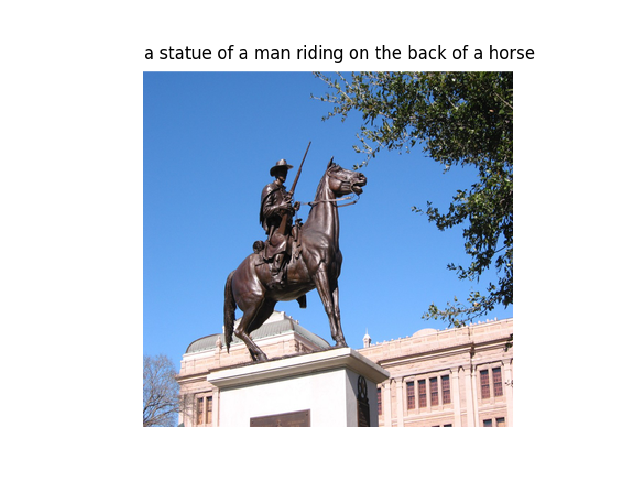
\includegraphics[width=80mm]{images/Figure_11.png}
\hspace*{-1cm}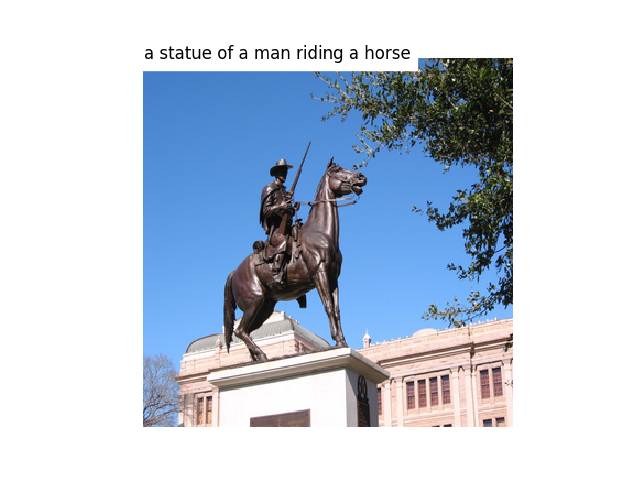
\includegraphics[width=80mm]{images/MFigure_11.png}
\hspace*{-1cm}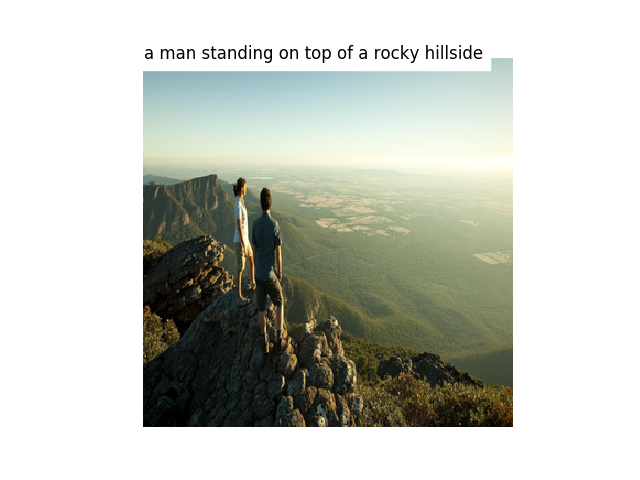
\includegraphics[width=80mm]{images/Figure_22.png}
\hspace*{-1cm}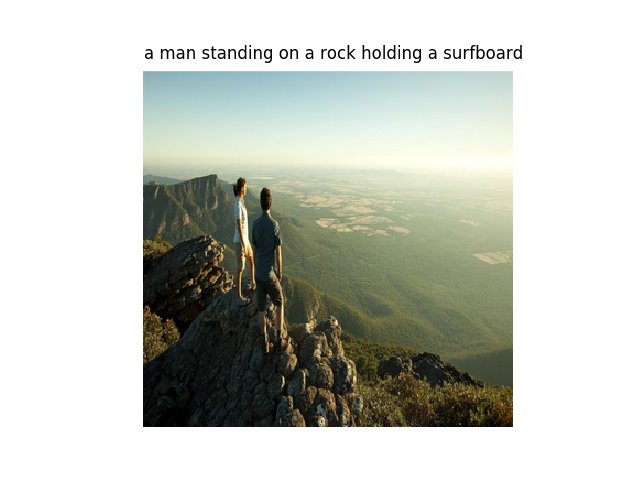
\includegraphics[width=80mm]{images/MFigure_22.png}
\hspace*{-1cm}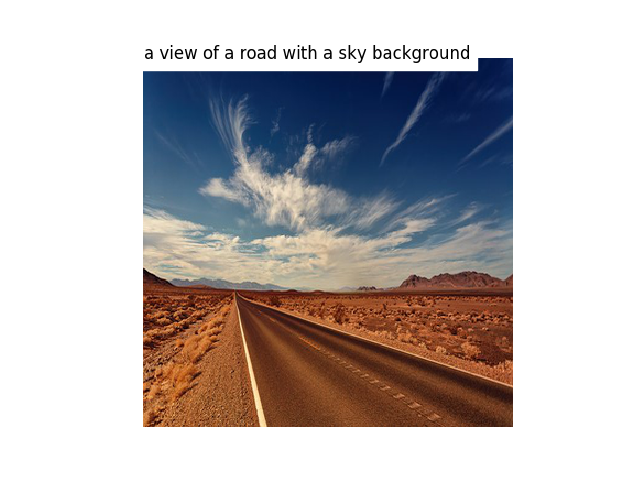
\includegraphics[width=80mm]{images/Figure_33.png}
\hspace*{-1cm}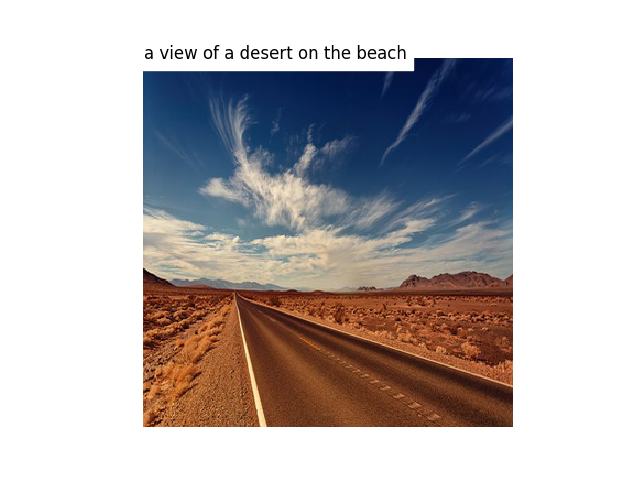
\includegraphics[width=80mm]{images/MFigure_33.png}
\hspace*{-1cm}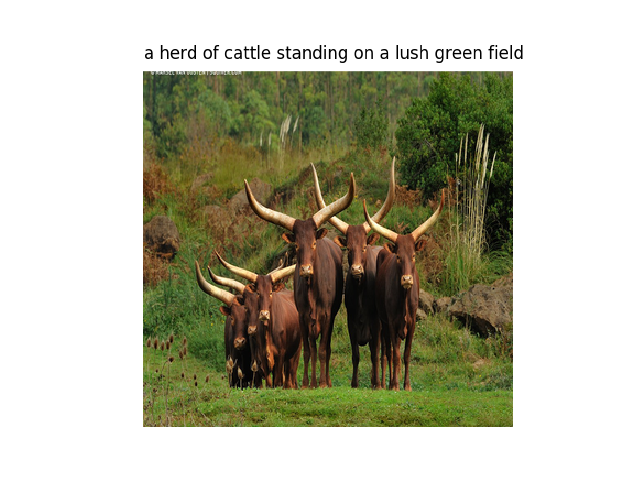
\includegraphics[width=80mm]{images/Figure_44.png}
\hspace*{-1cm}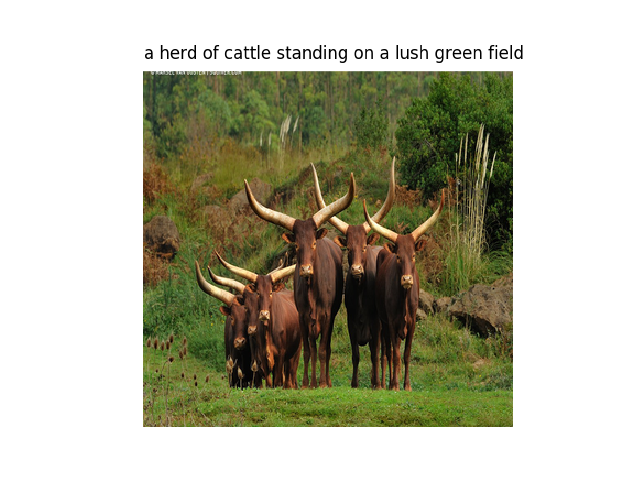
\includegraphics[width=80mm]{images/MFigure_44.png}
\hspace*{-1cm}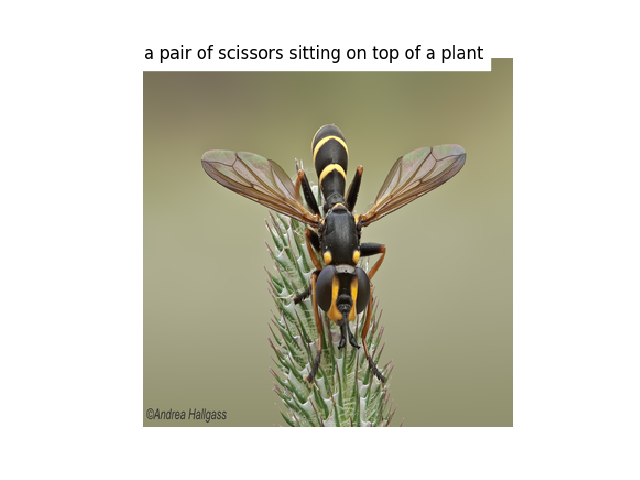
\includegraphics[width=80mm]{images/Figure_55.png}
\hspace*{-1cm}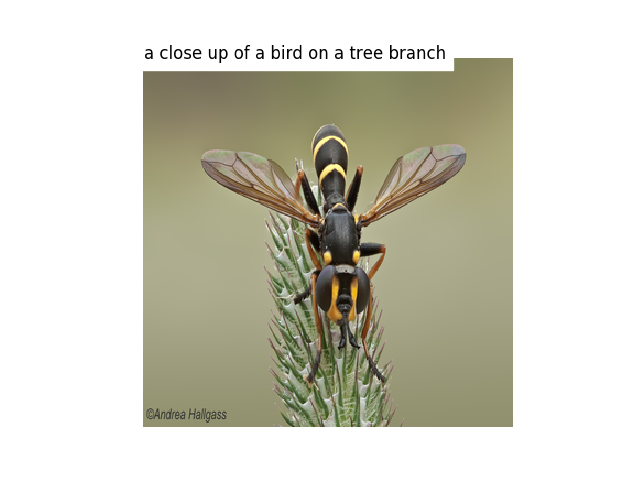
\includegraphics[width=80mm]{images/MFigure_55.png}
\hspace*{-1cm}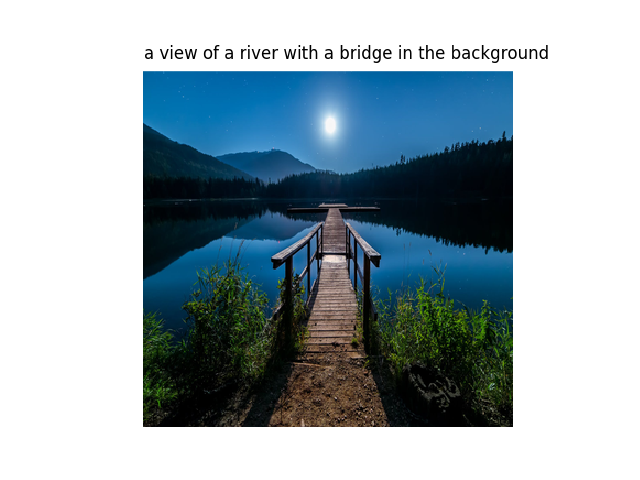
\includegraphics[width=80mm]{images/Figure_66.png}
\hspace*{-1cm}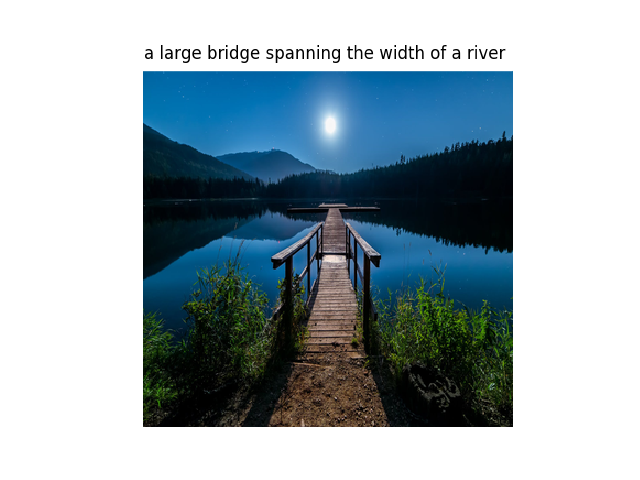
\includegraphics[width=80mm]{images/MFigure_66.png}

\end{document}


